\documentclass[]{article}
\usepackage{lmodern}
\usepackage{amssymb,amsmath}
\usepackage{ifxetex,ifluatex}
\usepackage{fixltx2e} % provides \textsubscript
\ifnum 0\ifxetex 1\fi\ifluatex 1\fi=0 % if pdftex
  \usepackage[T1]{fontenc}
  \usepackage[utf8]{inputenc}
\else % if luatex or xelatex
  \ifxetex
    \usepackage{mathspec}
  \else
    \usepackage{fontspec}
  \fi
  \defaultfontfeatures{Ligatures=TeX,Scale=MatchLowercase}
\fi
% use upquote if available, for straight quotes in verbatim environments
\IfFileExists{upquote.sty}{\usepackage{upquote}}{}
% use microtype if available
\IfFileExists{microtype.sty}{%
\usepackage{microtype}
\UseMicrotypeSet[protrusion]{basicmath} % disable protrusion for tt fonts
}{}
\usepackage[margin=1in]{geometry}
\usepackage{hyperref}
\PassOptionsToPackage{usenames,dvipsnames}{color} % color is loaded by hyperref
\hypersetup{unicode=true,
            pdftitle={Lab 03},
            colorlinks=true,
            linkcolor=Maroon,
            citecolor=Blue,
            urlcolor=Blue,
            breaklinks=true}
\urlstyle{same}  % don't use monospace font for urls
\usepackage{color}
\usepackage{fancyvrb}
\newcommand{\VerbBar}{|}
\newcommand{\VERB}{\Verb[commandchars=\\\{\}]}
\DefineVerbatimEnvironment{Highlighting}{Verbatim}{commandchars=\\\{\}}
% Add ',fontsize=\small' for more characters per line
\usepackage{framed}
\definecolor{shadecolor}{RGB}{248,248,248}
\newenvironment{Shaded}{\begin{snugshade}}{\end{snugshade}}
\newcommand{\AlertTok}[1]{\textcolor[rgb]{0.94,0.16,0.16}{#1}}
\newcommand{\AnnotationTok}[1]{\textcolor[rgb]{0.56,0.35,0.01}{\textbf{\textit{#1}}}}
\newcommand{\AttributeTok}[1]{\textcolor[rgb]{0.13,0.29,0.53}{#1}}
\newcommand{\BaseNTok}[1]{\textcolor[rgb]{0.00,0.00,0.81}{#1}}
\newcommand{\BuiltInTok}[1]{#1}
\newcommand{\CharTok}[1]{\textcolor[rgb]{0.31,0.60,0.02}{#1}}
\newcommand{\CommentTok}[1]{\textcolor[rgb]{0.56,0.35,0.01}{\textit{#1}}}
\newcommand{\CommentVarTok}[1]{\textcolor[rgb]{0.56,0.35,0.01}{\textbf{\textit{#1}}}}
\newcommand{\ConstantTok}[1]{\textcolor[rgb]{0.56,0.35,0.01}{#1}}
\newcommand{\ControlFlowTok}[1]{\textcolor[rgb]{0.13,0.29,0.53}{\textbf{#1}}}
\newcommand{\DataTypeTok}[1]{\textcolor[rgb]{0.13,0.29,0.53}{#1}}
\newcommand{\DecValTok}[1]{\textcolor[rgb]{0.00,0.00,0.81}{#1}}
\newcommand{\DocumentationTok}[1]{\textcolor[rgb]{0.56,0.35,0.01}{\textbf{\textit{#1}}}}
\newcommand{\ErrorTok}[1]{\textcolor[rgb]{0.64,0.00,0.00}{\textbf{#1}}}
\newcommand{\ExtensionTok}[1]{#1}
\newcommand{\FloatTok}[1]{\textcolor[rgb]{0.00,0.00,0.81}{#1}}
\newcommand{\FunctionTok}[1]{\textcolor[rgb]{0.13,0.29,0.53}{\textbf{#1}}}
\newcommand{\ImportTok}[1]{#1}
\newcommand{\InformationTok}[1]{\textcolor[rgb]{0.56,0.35,0.01}{\textbf{\textit{#1}}}}
\newcommand{\KeywordTok}[1]{\textcolor[rgb]{0.13,0.29,0.53}{\textbf{#1}}}
\newcommand{\NormalTok}[1]{#1}
\newcommand{\OperatorTok}[1]{\textcolor[rgb]{0.81,0.36,0.00}{\textbf{#1}}}
\newcommand{\OtherTok}[1]{\textcolor[rgb]{0.56,0.35,0.01}{#1}}
\newcommand{\PreprocessorTok}[1]{\textcolor[rgb]{0.56,0.35,0.01}{\textit{#1}}}
\newcommand{\RegionMarkerTok}[1]{#1}
\newcommand{\SpecialCharTok}[1]{\textcolor[rgb]{0.81,0.36,0.00}{\textbf{#1}}}
\newcommand{\SpecialStringTok}[1]{\textcolor[rgb]{0.31,0.60,0.02}{#1}}
\newcommand{\StringTok}[1]{\textcolor[rgb]{0.31,0.60,0.02}{#1}}
\newcommand{\VariableTok}[1]{\textcolor[rgb]{0.00,0.00,0.00}{#1}}
\newcommand{\VerbatimStringTok}[1]{\textcolor[rgb]{0.31,0.60,0.02}{#1}}
\newcommand{\WarningTok}[1]{\textcolor[rgb]{0.56,0.35,0.01}{\textbf{\textit{#1}}}}
\usepackage{graphicx,grffile}
\makeatletter
\def\maxwidth{\ifdim\Gin@nat@width>\linewidth\linewidth\else\Gin@nat@width\fi}
\def\maxheight{\ifdim\Gin@nat@height>\textheight\textheight\else\Gin@nat@height\fi}
\makeatother
% Scale images if necessary, so that they will not overflow the page
% margins by default, and it is still possible to overwrite the defaults
% using explicit options in \includegraphics[width, height, ...]{}
\setkeys{Gin}{width=\maxwidth,height=\maxheight,keepaspectratio}
\IfFileExists{parskip.sty}{%
\usepackage{parskip}
}{% else
\setlength{\parindent}{0pt}
\setlength{\parskip}{6pt plus 2pt minus 1pt}
}
\setlength{\emergencystretch}{3em}  % prevent overfull lines
\providecommand{\tightlist}{%
  \setlength{\itemsep}{0pt}\setlength{\parskip}{0pt}}
\setcounter{secnumdepth}{0}
% Redefines (sub)paragraphs to behave more like sections
\ifx\paragraph\undefined\else
\let\oldparagraph\paragraph
\renewcommand{\paragraph}[1]{\oldparagraph{#1}\mbox{}}
\fi
\ifx\subparagraph\undefined\else
\let\oldsubparagraph\subparagraph
\renewcommand{\subparagraph}[1]{\oldsubparagraph{#1}\mbox{}}
\fi

%%% Use protect on footnotes to avoid problems with footnotes in titles
\let\rmarkdownfootnote\footnote%
\def\footnote{\protect\rmarkdownfootnote}


  \title{Lab 03}
    \author{}
    \date{}
  

% change section title styling
\usepackage{sectsty}
\sectionfont{\normalsize\normalfont\itshape}
\subsectionfont{\normalsize\normalfont}

% use fancyhdr style
\usepackage{fancyhdr}
\pagestyle{fancy}
\fancyhead[LO, LE]{Lab 03}
\fancyhead[RO, RE]{Env Analysis in R}
\makeatletter
\renewcommand{\maketitle}{\bgroup\vspace*{-1cm}\setlength{\parindent}{0pt}
\begin{flushleft}
  \@author
  
  \@date
  
\end{flushleft}\egroup
}
\makeatother

\begin{document}
\maketitle

\section{Lab 03: Spatial autocorrelation, globally and
locally}\label{lab-03-spatial-autocorrelation-globally-and-locally}

\subsubsection{Read the instructions COMPLETELY before starting the
lab}\label{read-the-instructions-completely-before-starting-the-lab}

This lab builds on many of the discussions and exercises from class,
including previous labs.

\subsubsection{Attribution}\label{attribution}

This lab uses some code examples and directions from
\url{https://mgimond.github.io/Spatial/spatial-autocorrelation-in-r.html}

\subsubsection{Formatting your
submission}\label{formatting-your-submission}

This lab must be placed into a public repository on GitHub
(www.github.com). Before the due date, submit \textbf{on Canvas} a link
to the repository. I will then download your repositories and run your
code. The code must be contained in either a .R script or a .Rmd
markdown document. As I need to run your code, any data you use in the
lab must be referenced using \textbf{relative path names}. Finally,
answers to questions I pose in this document must also be in the
repository at the time you submit your link to Canvas. They can be in a
separate text file, or if you decide to use an RMarkdown document, you
can answer them directly in the doc.

\subsection{Data}\label{data}

The data for this lab can be found on the US Census website.

\begin{enumerate}
\def\labelenumi{\arabic{enumi}.}
\item
  First, go here:
  \url{https://www.census.gov/geographies/mapping-files/2020/geo/tiger-data.html}
\item
  Second, scroll to the ``Download Legal and Administrative Areas
  Geodatabases'' section
\item
  Click on ``County'' to download the county data for all of the US (the
  direct link is also here:
  \url{https://www2.census.gov/geo/tiger/TIGER_DP/2020ACS/ACS_2020_5YR_COUNTY.gdb.zip})
\end{enumerate}

\subsection{Introduction}\label{introduction}

In this lab, we will be calculating the spatial autocorrelation of
various Census variables across a subset of the US. Please note, the
dataset you downloaded above is larger than the current 100MB limit
GitHub imposes on single files. This means you'll be unable to push that
dataset to GitHub. Accordingly, I \emph{strongly} suggest you subset the
data such that your files are under this limit. This will be vital when
I grade your submissions. If you're not certain how to save a subset of
the file to disk, look at \texttt{?sf::write\_sf} for help. We will also
be using a new package called \texttt{spdep} in this assignment.

We begin by loading the relevant packages and data

\begin{Shaded}
\begin{Highlighting}[]
\FunctionTok{library}\NormalTok{(spdep)}
\end{Highlighting}
\end{Shaded}

\begin{verbatim}
## Warning: package 'spdep' was built under R version 4.4.1
\end{verbatim}

\begin{verbatim}
## Loading required package: spData
\end{verbatim}

\begin{verbatim}
## Warning: package 'spData' was built under R version 4.4.1
\end{verbatim}

\begin{verbatim}
## To access larger datasets in this package, install the spDataLarge
## package with: `install.packages('spDataLarge',
## repos='https://nowosad.github.io/drat/', type='source')`
\end{verbatim}

\begin{verbatim}
## Loading required package: sf
\end{verbatim}

\begin{verbatim}
## Warning: package 'sf' was built under R version 4.4.1
\end{verbatim}

\begin{verbatim}
## Linking to GEOS 3.11.0, GDAL 3.5.3, PROJ 9.1.0; sf_use_s2() is TRUE
\end{verbatim}

\begin{Shaded}
\begin{Highlighting}[]
\FunctionTok{library}\NormalTok{(sf)}
\FunctionTok{library}\NormalTok{(tidyverse)}
\end{Highlighting}
\end{Shaded}

\begin{verbatim}
## -- Attaching core tidyverse packages ------------------------ tidyverse 2.0.0 --
## v dplyr     1.1.4     v readr     2.1.5
## v forcats   1.0.0     v stringr   1.5.1
## v ggplot2   3.5.1     v tibble    3.2.1
## v lubridate 1.9.3     v tidyr     1.3.1
## v purrr     1.0.2
\end{verbatim}

\begin{verbatim}
## -- Conflicts ------------------------------------------ tidyverse_conflicts() --
## x dplyr::filter() masks stats::filter()
## x dplyr::lag()    masks stats::lag()
## i Use the conflicted package (<http://conflicted.r-lib.org/>) to force all conflicts to become errors
\end{verbatim}

\begin{Shaded}
\begin{Highlighting}[]
\FunctionTok{library}\NormalTok{(tmap)}
\end{Highlighting}
\end{Shaded}

\begin{verbatim}
## Warning: package 'tmap' was built under R version 4.4.1
\end{verbatim}

Next, we load our data, look at it, then maybe plot it (the plot might
take some time). This file is a geodatabase, a proprietary file format
created by ESRI. Conveniently, \texttt{sf\_read} can actually read
geodatabases. However, we also have to know the layer name ahead of
time.

First, let's read the layer that has the geometry in this gdb file.

\begin{Shaded}
\begin{Highlighting}[]
\NormalTok{d.all }\OtherTok{\textless{}{-}}\NormalTok{ sf}\SpecialCharTok{::}\FunctionTok{read\_sf}\NormalTok{(}\StringTok{"../data/ACS\_2020\_5YR\_COUNTY.gdb"}\NormalTok{, }\AttributeTok{layer =} \StringTok{"ACS\_2020\_5YR\_COUNTY"}\NormalTok{)}
\FunctionTok{glimpse}\NormalTok{(d.all)}
\end{Highlighting}
\end{Shaded}

\begin{verbatim}
## Rows: 3,221
## Columns: 21
## $ STATEFP      <chr> "31", "53", "35", "31", "31", "72", "46", "48", "06", "21~
## $ COUNTYFP     <chr> "039", "069", "011", "109", "129", "085", "099", "327", "~
## $ COUNTYNS     <chr> "00835841", "01513275", "00933054", "00835876", "00835886~
## $ GEOID        <chr> "31039", "53069", "35011", "31109", "31129", "72085", "46~
## $ NAME         <chr> "Cuming", "Wahkiakum", "De Baca", "Lancaster", "Nuckolls"~
## $ NAMELSAD     <chr> "Cuming County", "Wahkiakum County", "De Baca County", "L~
## $ LSAD         <chr> "06", "06", "06", "06", "06", "13", "06", "06", "06", "06~
## $ CLASSFP      <chr> "H1", "H1", "H1", "H1", "H1", "H1", "H1", "H1", "H1", "H1~
## $ MTFCC        <chr> "G4020", "G4020", "G4020", "G4020", "G4020", "G4020", "G4~
## $ CSAFP        <chr> " ", " ", " ", "339", " ", "490", " ", " ", " ", " ", "53~
## $ CBSAFP       <chr> " ", " ", " ", "30700", " ", "41980", "43620", " ", " ", ~
## $ METDIVFP     <chr> " ", " ", " ", " ", " ", " ", " ", " ", " ", " ", " ", " ~
## $ FUNCSTAT     <chr> "A", "A", "A", "A", "A", "A", "A", "A", "A", "A", "A", "A~
## $ ALAND        <dbl> 1477645345, 680976231, 6016818946, 2169272970, 1489645188~
## $ AWATER       <dbl> 10690204, 61568965, 29090018, 22847034, 1718484, 32509, 1~
## $ INTPTLAT     <chr> "+41.9158651", "+46.2946377", "+34.3592729", "+40.7835474~
## $ INTPTLON     <chr> "-096.7885168", "-123.4244583", "-104.3686961", "-096.688~
## $ Shape_Length <dbl> 1.6244323, 1.4491768, 3.4551326, 1.9433801, 1.6022818, 0.~
## $ Shape_Area   <dbl> 0.161522931, 0.086692186, 0.592344046, 0.233861880, 0.157~
## $ GEOID_Data   <chr> "05000US31039", "05000US53069", "05000US35011", "05000US3~
## $ Shape        <MULTIPOLYGON [°]> MULTIPOLYGON (((-97.01952 4..., MULTIPOLYGON~
\end{verbatim}

\begin{Shaded}
\begin{Highlighting}[]
\CommentTok{\#tmap::tm\_shape(d.all) + tm\_polygons() \# commented out because }
\CommentTok{\#it\textquotesingle{}s a large dataset that takes a long time to plot}
\end{Highlighting}
\end{Shaded}

Next, we're going to read the geodatabase again, but this time a
tablular dataset containing age and sex data. Because the GEOID in this
table and in the geometry file are different, we need to create a geoid
in this table that will match.

\begin{Shaded}
\begin{Highlighting}[]
\NormalTok{d.x1 }\OtherTok{\textless{}{-}}\NormalTok{ sf}\SpecialCharTok{::}\FunctionTok{read\_sf}\NormalTok{(}\StringTok{"../data/ACS\_2020\_5YR\_COUNTY.gdb"}\NormalTok{, }\AttributeTok{layer =} \StringTok{"X01\_AGE\_AND\_SEX"}\NormalTok{) }\SpecialCharTok{\%\textgreater{}\%}
  \FunctionTok{mutate}\NormalTok{(}\AttributeTok{fixed\_geoid =} \FunctionTok{str\_sub}\NormalTok{(GEOID, }\AttributeTok{start =} \DecValTok{8}\NormalTok{, }\AttributeTok{end =} \SpecialCharTok{{-}}\DecValTok{1}\NormalTok{)) }
\CommentTok{\# the {-}1 is a shortcut to tell R to go to the end of the string}
\end{Highlighting}
\end{Shaded}

Finally, we're going to join the tabular and spatial data together.

\begin{Shaded}
\begin{Highlighting}[]
\NormalTok{d.joined }\OtherTok{\textless{}{-}}\NormalTok{ d.all }\SpecialCharTok{\%\textgreater{}\%} \FunctionTok{left\_join}\NormalTok{(., d.x1, }\AttributeTok{by =} \FunctionTok{c}\NormalTok{(}\StringTok{"GEOID"} \OtherTok{=} \StringTok{"fixed\_geoid"}\NormalTok{))}
\end{Highlighting}
\end{Shaded}

Again, the data are too large, so we need to creat a subset we can work
with later. Let's use the GEOID to create a dataset with only those
counties in Ohio Be sure to check the data type of GEOID.

\begin{Shaded}
\begin{Highlighting}[]
\CommentTok{\# get just Ohio}
\NormalTok{ohio }\OtherTok{\textless{}{-}}\NormalTok{ d.joined }\SpecialCharTok{\%\textgreater{}\%}\NormalTok{ dplyr}\SpecialCharTok{::}\FunctionTok{filter}\NormalTok{(STATEFP }\SpecialCharTok{==} \StringTok{"39"}\NormalTok{)}


\CommentTok{\# map it to verify}
\NormalTok{tmap}\SpecialCharTok{::}\FunctionTok{tm\_shape}\NormalTok{(ohio) }\SpecialCharTok{+} \FunctionTok{tm\_polygons}\NormalTok{()}
\end{Highlighting}
\end{Shaded}

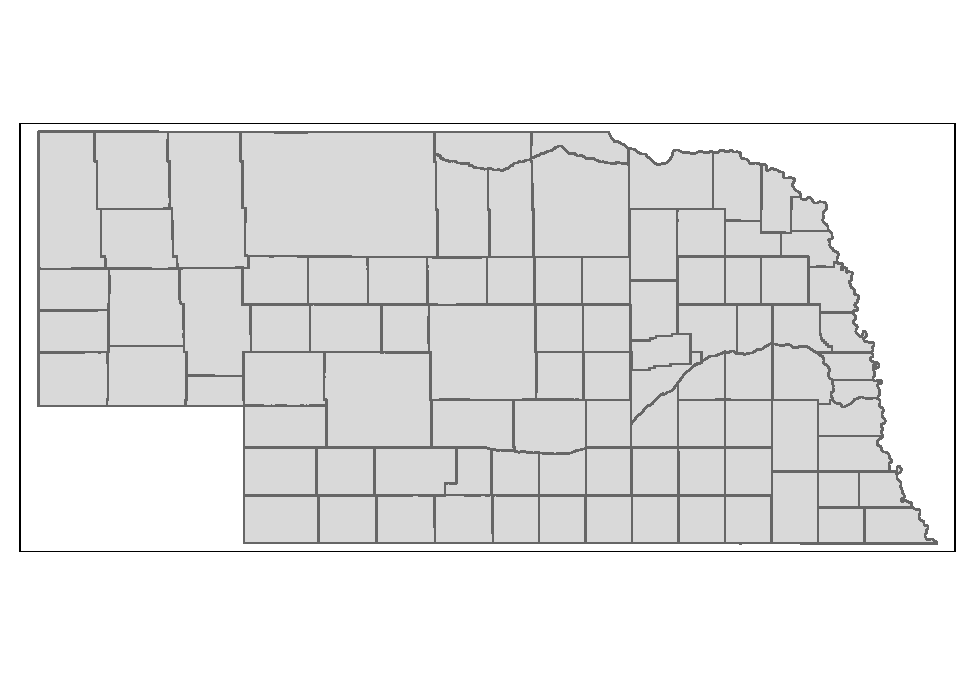
\includegraphics{lab03_files/figure-latex/make_subset-1.pdf}

Next, we'll formalize our space by creating neighbors, and thus,
\textbf{W}

\begin{itemize}
\tightlist
\item
  First we'll project
\item
  Next, we'll use Queen contiguity to define \textbf{W}
\end{itemize}

\begin{Shaded}
\begin{Highlighting}[]
\CommentTok{\# Check it first}
\NormalTok{sf}\SpecialCharTok{::}\FunctionTok{st\_crs}\NormalTok{(ohio) }
\end{Highlighting}
\end{Shaded}

\begin{verbatim}
## Coordinate Reference System:
##   User input: NAD83 
##   wkt:
## GEOGCRS["NAD83",
##     DATUM["North American Datum 1983",
##         ELLIPSOID["GRS 1980",6378137,298.257222101,
##             LENGTHUNIT["metre",1]]],
##     PRIMEM["Greenwich",0,
##         ANGLEUNIT["degree",0.0174532925199433]],
##     CS[ellipsoidal,2],
##         AXIS["geodetic latitude (Lat)",north,
##             ORDER[1],
##             ANGLEUNIT["degree",0.0174532925199433]],
##         AXIS["geodetic longitude (Lon)",east,
##             ORDER[2],
##             ANGLEUNIT["degree",0.0174532925199433]],
##     USAGE[
##         SCOPE["Geodesy."],
##         AREA["North America - onshore and offshore: Canada - Alberta; British Columbia; Manitoba; New Brunswick; Newfoundland and Labrador; Northwest Territories; Nova Scotia; Nunavut; Ontario; Prince Edward Island; Quebec; Saskatchewan; Yukon. Puerto Rico. United States (USA) - Alabama; Alaska; Arizona; Arkansas; California; Colorado; Connecticut; Delaware; Florida; Georgia; Hawaii; Idaho; Illinois; Indiana; Iowa; Kansas; Kentucky; Louisiana; Maine; Maryland; Massachusetts; Michigan; Minnesota; Mississippi; Missouri; Montana; Nebraska; Nevada; New Hampshire; New Jersey; New Mexico; New York; North Carolina; North Dakota; Ohio; Oklahoma; Oregon; Pennsylvania; Rhode Island; South Carolina; South Dakota; Tennessee; Texas; Utah; Vermont; Virginia; Washington; West Virginia; Wisconsin; Wyoming. US Virgin Islands. British Virgin Islands."],
##         BBOX[14.92,167.65,86.45,-40.73]],
##     ID["EPSG",4269]]
\end{verbatim}

\begin{Shaded}
\begin{Highlighting}[]
\CommentTok{\# then reproject to north american equidistant conic}
\NormalTok{ohio.projected }\OtherTok{\textless{}{-}}\NormalTok{ ohio }\SpecialCharTok{\%\textgreater{}\%}\NormalTok{ sf}\SpecialCharTok{::}\FunctionTok{st\_transform}\NormalTok{(., }\StringTok{"ESRI:102010"}\NormalTok{)}

\CommentTok{\# plot it again to make sure nothing broke}
\NormalTok{tmap}\SpecialCharTok{::}\FunctionTok{tm\_shape}\NormalTok{(ohio.projected) }\SpecialCharTok{+} \FunctionTok{tm\_polygons}\NormalTok{()}
\end{Highlighting}
\end{Shaded}

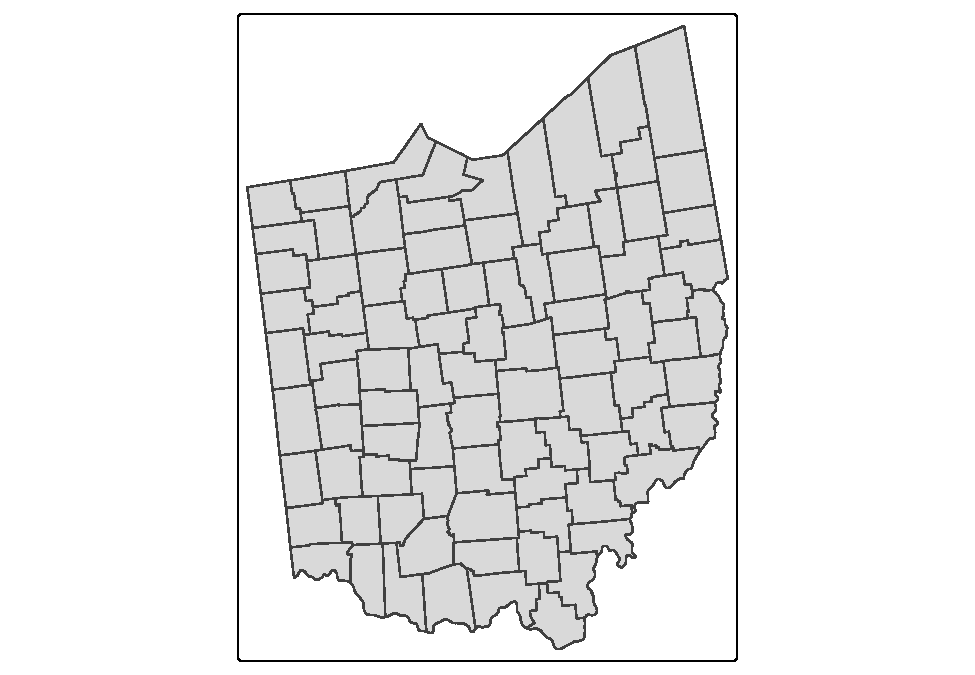
\includegraphics{lab03_files/figure-latex/make some neighbors-1.pdf}

\begin{Shaded}
\begin{Highlighting}[]
\CommentTok{\# make the neighborhood}
\NormalTok{nb }\OtherTok{\textless{}{-}}\NormalTok{ spdep}\SpecialCharTok{::}\FunctionTok{poly2nb}\NormalTok{(ohio.projected, }\AttributeTok{queen =} \ConstantTok{TRUE}\NormalTok{)}
\end{Highlighting}
\end{Shaded}

For each polygon in our polygon object, \texttt{nb} lists all
neighboring polygons. For example, to see the neighbors for the first
polygon in the object, type:

\begin{Shaded}
\begin{Highlighting}[]
\NormalTok{nb[[}\DecValTok{1}\NormalTok{]]}
\end{Highlighting}
\end{Shaded}

\begin{verbatim}
## [1]  2 11 66 69 73 74 87
\end{verbatim}

Polygon 1 has 4 neighbors. The numbers represent the polygon IDs as
stored in the spatial object \texttt{ohio.projected}. Polygon 1 is
associated with the County attribute name \texttt{"Hancock\ County"} and
its four neighboring polygons are associated with the counties:

\begin{Shaded}
\begin{Highlighting}[]
\NormalTok{ohio.projected}\SpecialCharTok{$}\NormalTok{NAMELSAD[}\DecValTok{1}\NormalTok{] }\CommentTok{\# county in index 1}
\end{Highlighting}
\end{Shaded}

\begin{verbatim}
## [1] "Hancock County"
\end{verbatim}

\begin{Shaded}
\begin{Highlighting}[]
\NormalTok{nb[[}\DecValTok{1}\NormalTok{]] }\SpecialCharTok{\%\textgreater{}\%}\NormalTok{ ohio.projected}\SpecialCharTok{$}\NormalTok{NAMELSAD[.] }\CommentTok{\# and it\textquotesingle{}s neighbors. }
\end{Highlighting}
\end{Shaded}

\begin{verbatim}
## [1] "Allen County"   "Henry County"   "Hardin County"  "Putnam County" 
## [5] "Wood County"    "Seneca County"  "Wyandot County"
\end{verbatim}

\begin{Shaded}
\begin{Highlighting}[]
\CommentTok{\# Note we\textquotesingle{}re doing this programmatically step{-}by{-}step}
\end{Highlighting}
\end{Shaded}

Next, we need to assign weights to each neighboring polygon. In our
case, each neighboring polygon will be assigned equal weight
\texttt{(style="W")}. This is accomplished by assigning the fraction:
\texttt{1\ /\ (\ \#\ of\ neighbors)} to each neighboring county then
summing the weighted values. While this is the most intuitive way to
summaries the neighbors' values it has one drawback in that polygons
along the edges of the study area will base their lagged values on fewer
polygons thus potentially over- or under-estimating the true nature of
the spatial autocorrelation in the data. For this example, we'll stick
with the \texttt{style="W"} option for simplicity's sake but note that
other more robust options are available, notably \texttt{style="B"}.

\begin{Shaded}
\begin{Highlighting}[]
\NormalTok{lw }\OtherTok{\textless{}{-}} \FunctionTok{nb2listw}\NormalTok{(nb, }\AttributeTok{style=}\StringTok{"W"}\NormalTok{, }\AttributeTok{zero.policy=}\ConstantTok{TRUE}\NormalTok{)}
\end{Highlighting}
\end{Shaded}

The \texttt{zero.policy=TRUE} option allows for lists of non-neighbors.
This should be used with caution since the user may not be aware of
missing neighbors in their dataset. However, a zero.policy of
\texttt{FALSE} would return an error if you have a dataset where a
polygon does not have a neighbor.

To see the weight of the first polygon's four neighbors type:

\begin{Shaded}
\begin{Highlighting}[]
\NormalTok{lw}\SpecialCharTok{$}\NormalTok{weights[}\DecValTok{1}\NormalTok{]}
\end{Highlighting}
\end{Shaded}

\begin{verbatim}
## [[1]]
## [1] 0.1428571 0.1428571 0.1428571 0.1428571 0.1428571 0.1428571 0.1428571
\end{verbatim}

This row-normalized our weights!

We can also plot the distribution of neighbors across the dataset.

\begin{Shaded}
\begin{Highlighting}[]
\CommentTok{\# use attr to get the count of neighbors in W}
\NormalTok{neighbors }\OtherTok{\textless{}{-}} \FunctionTok{attr}\NormalTok{(lw}\SpecialCharTok{$}\NormalTok{weights,}\StringTok{"comp"}\NormalTok{)}\SpecialCharTok{$}\NormalTok{d }

\CommentTok{\# plot it}
\FunctionTok{hist}\NormalTok{(neighbors)}
\end{Highlighting}
\end{Shaded}

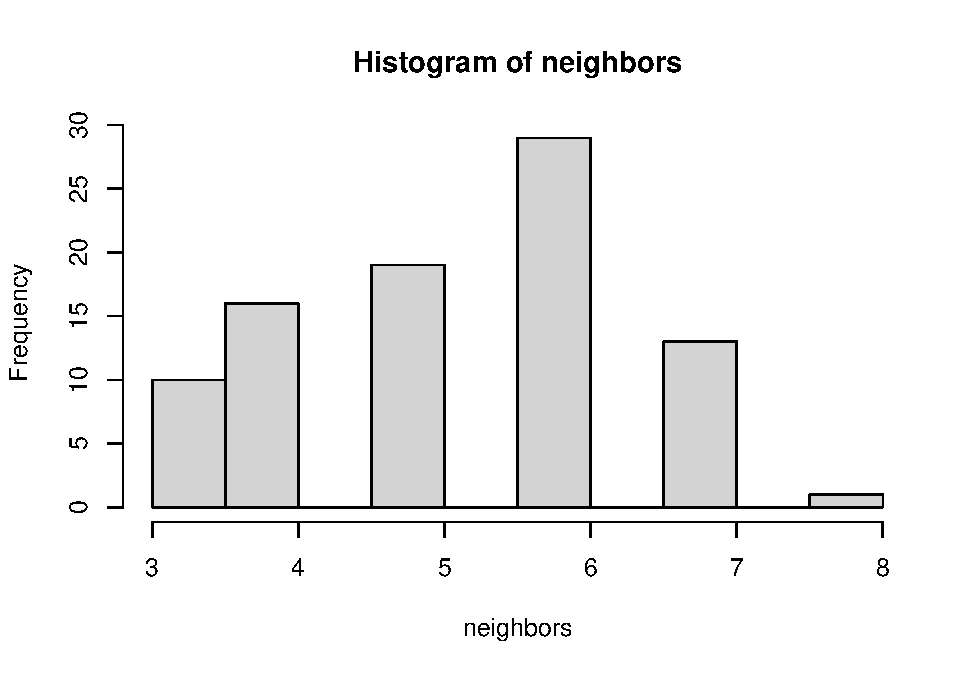
\includegraphics{lab03_files/figure-latex/plotneighbors-1.pdf}

Finally, we'll compute the average neighbor population of Females 75-79
years of age for each polygon. These values are often referred to as
spatially lagged values. The following table shows the average
neighboring F 75-79 values (stored in the F75.lag object) for each
county. Note, I deterimined the correct attribute (B01001e47) by reading
the metadata from the original Census Bureau link

\begin{Shaded}
\begin{Highlighting}[]
\NormalTok{F75.lag }\OtherTok{\textless{}{-}} \FunctionTok{lag.listw}\NormalTok{(lw, ohio.projected}\SpecialCharTok{$}\NormalTok{B01001e47)}
\NormalTok{F75.lag}
\end{Highlighting}
\end{Shaded}

\begin{verbatim}
##  [1]  929.0000  748.8000 9055.0000 1264.3333 6629.7500  944.0000 8303.3333
##  [8]  699.5000  771.1667  695.0000 1836.8571 2679.6667 1271.2500  732.8000
## [15] 2779.5000  987.8000  970.0000  840.6667  879.7500 1013.5000  941.0000
## [22]  835.0000 3368.3333  903.5000  912.4000 1296.6667 4114.4000 2805.5000
## [29] 1186.2000 3279.0000 1100.6667 3066.0000 3428.8333 2893.2000 2881.6667
## [36] 2057.5714 1022.7500 3480.3333 5395.6667  917.0000 2850.1250 3981.2500
## [43] 1667.8333  783.1667 1592.0000  938.5000 1397.6667 1958.2500 1838.6667
## [50] 5989.0000  574.7500  612.6667  976.7500 1233.4000 2476.0000  905.3333
## [57] 7564.5000 3753.0000 2263.1667 3469.2500 2547.6000  656.6000  585.4286
## [64]  442.7500 3231.7143  978.7143 4372.0000  936.1667 1060.1429  550.0000
## [71] 1684.6667 1798.1429 1710.2857 1084.5000  683.0000 3039.2857 4302.5000
## [78] 5727.1667 3893.2000 1492.7143 3305.2857 6667.0000 1061.0000 8028.2000
## [85]  599.7500 1390.6667  945.4000  864.7500
\end{verbatim}

\subsubsection{Computing Moran's I}\label{computing-morans-i}

To get the Moran's I value, simply use the moran.test function.

\begin{Shaded}
\begin{Highlighting}[]
\FunctionTok{moran.test}\NormalTok{(ohio.projected}\SpecialCharTok{$}\NormalTok{B01001e47, lw)}
\end{Highlighting}
\end{Shaded}

\begin{verbatim}
## 
##  Moran I test under randomisation
## 
## data:  ohio.projected$B01001e47  
## weights: lw    
## 
## Moran I statistic standard deviate = 3.7465, p-value = 8.966e-05
## alternative hypothesis: greater
## sample estimates:
## Moran I statistic       Expectation          Variance 
##        0.20527330       -0.01149425        0.00334761
\end{verbatim}

Note that the p-value computed from the \texttt{moran.test} function is
not computed from an MC simulation but \textbf{analytically} instead.
This may not always prove to be the most accurate measure of
significance. To test for significance using the MC simulation method
instead, use the moran.mc function.

\subsubsection{Moran's plots}\label{morans-plots}

Thus far, our analysis has been a global investigation of spatial
autocorrelation. We can also use local indicators of spatial
autocorrelation (LISA) to analyze our dataset. One way of doing so is
through the use of a Moran plot.

The process to make a plot is relatively simple:

\begin{Shaded}
\begin{Highlighting}[]
\CommentTok{\# use zero.policy = T because some polygons don\textquotesingle{}t have neighbors}
\FunctionTok{moran.plot}\NormalTok{(ohio.projected}\SpecialCharTok{$}\NormalTok{B01001e47, lw, }\AttributeTok{zero.policy=}\ConstantTok{TRUE}\NormalTok{, }\AttributeTok{plot=}\ConstantTok{TRUE}\NormalTok{)}
\end{Highlighting}
\end{Shaded}

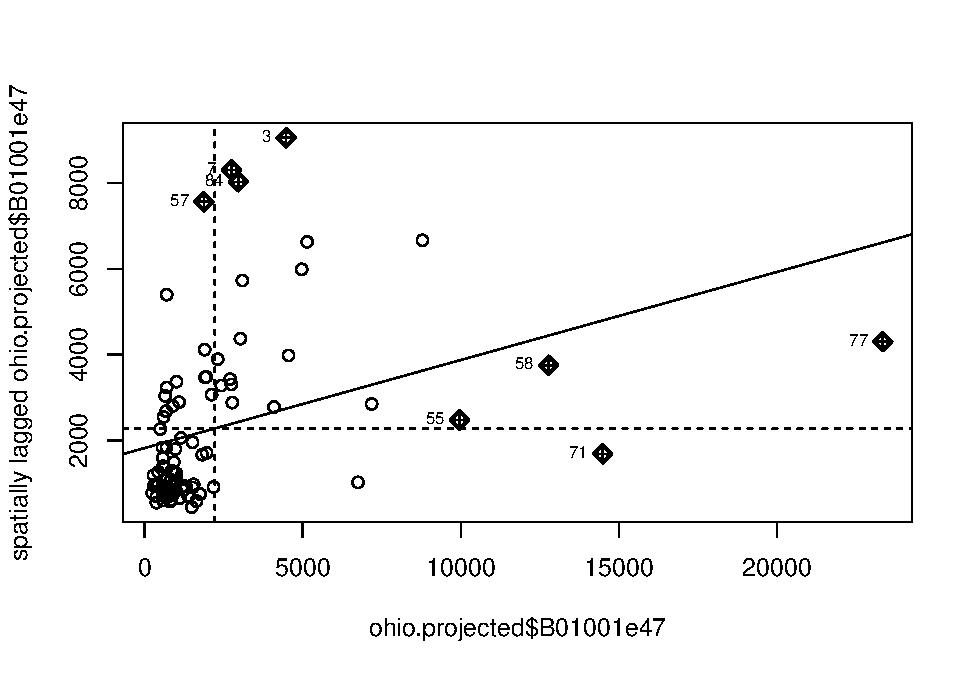
\includegraphics{lab03_files/figure-latex/moranplot-1.pdf}

\subsection{Your tasks}\label{your-tasks}

\begin{enumerate}
\def\labelenumi{\arabic{enumi}.}
\item
  Create a spatial subset of the US, with at AT MINIMUM 4 states,
  MAXIMUM 7 states. States must be contiguous. Save this subset as a
  shapefile such that it's sufficiently small in size that GitHub will
  accept the git-push
\item
  Choose a variable. If it's a raw count, you should normalize the
  variable in an appropriate manner (e.g., by total population, percent,
  by area)
\item
  Make a histogram of your chosen variable
\item
  Make a choropleth map of your chosen variable. Choose an appropriate
  data classification scheme
\item
  Develop a contiguity-based spatial weights matrix of your choosing
  (i.e., rook or queen)
\item
  Row-standardize the W
\item
  Plot a histogram of the number of neighbors
\item
  Calculate the average number of neighbors
\item
  Make a Moran Plot
\item
  Repeat \#5 (and 5.1 - 5.4) above with a W developed using the IDW
  method. You will need to investigate the \texttt{spdep} documentation
  to find the correct method/function.
\end{enumerate}

\subsection{Questions:}\label{questions}

\begin{enumerate}
\def\labelenumi{\arabic{enumi}.}
\item
  Describe in your own words how Moran's I is calculated
\item
  Describe in your own words: what is a spatially-lagged variable?
\item
  How does your analysis in this lab (as simple as it is) diffr by how
  you have formalized W (e.g., space, neighbors) in two different
  methods? How might it affect analysis?
\item
  What does it mean if an observation falls in the ``H-L'' quadrant? Why
  might it be useful to detect such occurances?
\end{enumerate}

\subsection{Bonus (+50 points)}\label{bonus-50-points}

B1. make another Moran plot, this time do so manually (use
\texttt{geom\_point} from \texttt{ggplot}). You must label each quadrant
with HH, HL, LL, and LH, respectively. You should also use color and/or
shape to denote whether an observation is statistically significant.
Tip, you can find the data you want using the \texttt{moran.plot}
function, but you'll have to alter the function call and read some
documentation.

B2. plot a choropleth map of your dataset with a categorical color
scheme, where the shading corresponds to the Moran plot (really,
``LISA'') quadrants. Thus, your map will have four shades of color.


\end{document}